\documentclass[final]{beamer}
\usetheme{summer}
\setbeamerfont{itemize}{size=\normalsize}
\setbeamerfont{itemize/enumerate body}{size=\normalsize}
\setbeamerfont{itemize/enumerate subbody}{size=\normalsize}
\usepackage[english]{babel}
\usepackage[latin1]{inputenc}
\usepackage{amsmath} %and any other packages upon which you call
\usefonttheme[onlymath]{serif}
\usepackage[orientation=landscape,size=a0,scale=1.4]{beamerposter}
\title{Block! and related puzzles}
\author{Patrick Stevens}
\begin{document}
\vspace{2\baselineskip}
\begin{columns}[t]
\begin{column}{.3 \linewidth}

\begin{block}{Block!}\ \\
Block! is a puzzle game, where the aim is to tile a board with polyominoes.\\~\\

\begin{center}
% Picture of a Block! instance
\includegraphics[width=0.3 \linewidth]{block}
\end{center}

The picture shows a partially-completed puzzle.

We may view Block! as a tree exploration problem: moving from the empty board state to a full board state, via intermediate states which are obtained by placing a piece.
\end{block}
\vspace{\baselineskip}

\begin{block}{Doors!}\ \\
Doors! is an abstraction which is meant to capture the tree-like nature of Block!
We are in a room, and see three doors ahead.
Each door has a probability marked on it, reflecting our confidence that that path will lead to a solution.
Once we go through a door, we see a sign in the new room, with a new probability on it: a better estimate of the probability that a solution lies this way.
The idea is to find a solution in the most efficient way possible, updating our probabilities as we go.\\~\\

\begin{center}
% Picture of a Doors! graph
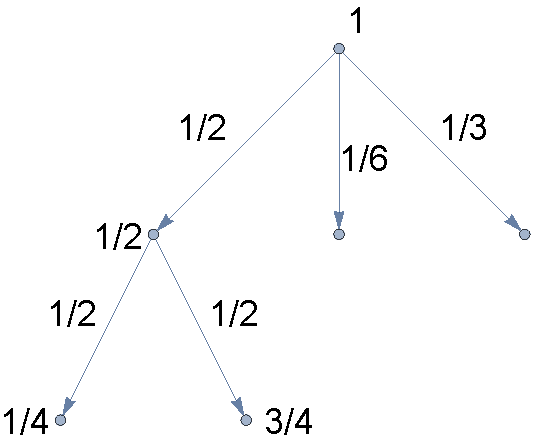
\includegraphics[width=0.25 \linewidth]{doorsgraph}
\end{center}

The fact that ``the room probability is not the same as the door probability'' reflects the fact that humans are not very good at visualising the future board state.
We may put a Block! piece into the board, and immediately realise that we've done something stupid, and remove the piece again.
That would correspond to going through a high-probability door and seeing a low-probability sign in the new room. \\~\\

There are some technical difficulties in defining Doors! puzzles, in saying what the probabilities actually mean in the presence of partial information, and in updating our probabilities correctly.
\end{block}
\end{column}

% ----- column 2
\begin{column}{.3 \linewidth}

\begin{block}{Doors! Unlimited}\ \\
Doors! Unlimited is an infinitised version of Doors!, which avoids some of the technical difficulties.
It takes place on an infinite graph which is homogeneous in some way.
Instead of assessing probabilities of a path, each node has a piece of treasure in with probability $p$ independently.
Each door has a time-cost associated with it, and we want to find $k$ pieces of treasure in the least time down a single path. \\~\\

\begin{center}
% Picture of a Doors! Unlimited graph
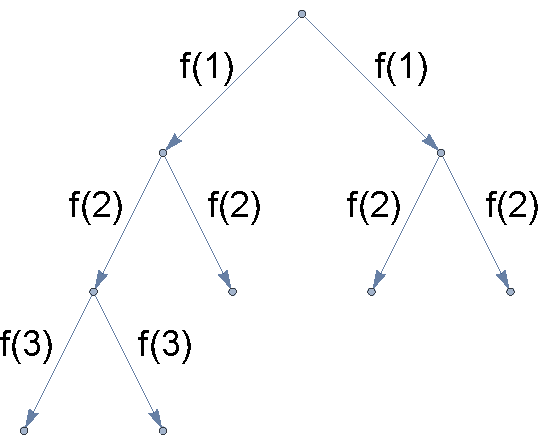
\includegraphics[width=0.25 \linewidth]{doorsunlimitedgraph}
\end{center}

Assume the time-cost function $f$ is increasing to infinity as depth goes to infinity, and is equal for all doors on the same level.

Then Doors! Unlimited is an infinite Markov process, but given these restrictions on $f$, there are theorems which assure us that optimal strategies exist. \\~\\

Doors! Unlimited has the advantage that it is very precisely defined what every quantity of interest really means, and the update procedure is totally unambiguous.
However, the cost of a strategy is very sensitive to the order in which we open doors, which makes analysis quite hard.
\end{block}
\vspace{\baselineskip}


\begin{block}{CorriDoors!}\ \\
CorriDoors! is a specific version of Doors! Unlimited.
It takes place on two rooted infinite unary trees, and is easy to picture. \\~\\

\begin{center}
% Picture of CorriDoors! puzzle
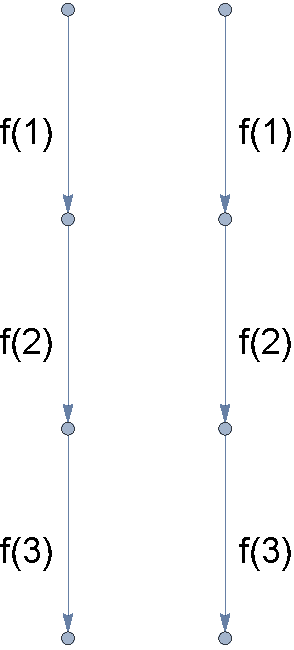
\includegraphics[width=0.09 \linewidth]{corridoorsgraph}
\end{center}
\end{block}
\vspace{\baselineskip}

\begin{block}{Obvious things we can say}\ \\
We can see many easy things which are hard to prove.
For example, if we haven't found any coins so far, but we've explored further down the left path, then we want to go down the right next, because it's cheaper. \\~\\
This is intuitively obvious, but in fact the strongest result we proved here is that there are only finitely many instances in which it's better to take the deeper door.
(We want ``finitely many'' to be ``none''.)
\end{block}
\vspace{\baselineskip}


\end{column}

% -------column 3-------

\begin{column}{.3 \linewidth}

\begin{block}{Example case: one coin to find}\ \\
Suppose $k=1$: that is, one coin left to find.
We can prove that it's optimal to do the obvious thing: to go down the shallowest path at each stage.
Actually, we can do better: this is true even for the more general Doors! Unlimited. \\~\\

The way we do this is to show that if we ever take the deeper door before a shallower door, we can improve our expected time-cost by deferring taking the deep door for a turn.
Then by induction, the optimal cost is achieved when the shallowest doors are taken first. \\~\\

\begin{center}
% Picture of CorriDoors! with only one coin left to find
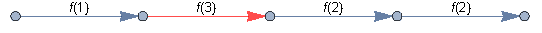
\includegraphics[width=0.5 \linewidth]{corridoors1} \\
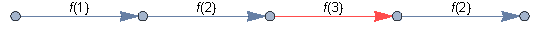
\includegraphics[width=0.5 \linewidth]{corridoors2} \\
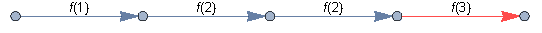
\includegraphics[width=0.5 \linewidth]{corridoors3}
\end{center}

However, this proof relies heavily on the one-coin-left condition.
If the game might not terminate once we've found a coin, everything becomes highly recursive and difficult to study.

%\begin{center}
% % Picture of CorriDoors! with only one coin left to find
%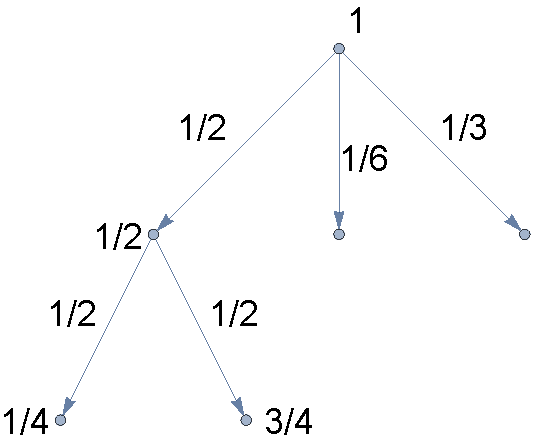
\includegraphics[width=0.5 \linewidth]{doorsgraph}
%\end{center}

\end{block}
\vspace{\baselineskip}

\vspace{\baselineskip}

\begin{block}{Conjecture 8}\ \\

Back on Doors! Unlimited, we have a conjecture which is intuitive and would tell us a lot about these obvious situations. \\~\\

%\begin{center}
% % Picture of a Doors! Unlimited instance where we remove a vertex
%\includegraphics[width=0.5 \linewidth]{removing_optimal_vertex}
%\end{center}

We say the \emph{optimal set} $\mathcal{O}(D)$ of a position $D$ is the set of all doors which have an optimal strategy beginning with that door.
Then Conjecture 8 states that removing a door $d$ from the non-optimal set won't change the optimal set, and that removing a non-unique optimal door won't change the optimal set much.
That is,

\vspace{\baselineskip}

\[ \begin{cases} 
      \mathcal{O}(D) & : \text{$d \not \in \mathcal{O}(D)$} \\
      \mathcal{O}(D) \setminus \{ d \} & : \text{$d \in \mathcal{O}(D) \not = \{ d \}$}
   \end{cases}
\] \\~\\

\vspace{\baselineskip}

This conjecture would let us prove things about the optimal sets in Doors! Unlimited instances by induction.
We have made partial progress in proving it (we can nearly show that each case of behaviour is equivalent to the other), and we have made partial progress in proving other intuitive results given this one.
For instance, the ``shallowest door is optimal'' result from CorriDoors! is enough to prove it for general Doors! Unlimited cases in the presence of Conjecture 8.

\end{block}
\vspace{\baselineskip}

\end{column}

\end{columns}
\end{document}